\documentclass[
  bibliography=totoc,     % Literatur im Inhaltsverzeichnis
  captions=tableheading,  % Tabellenüberschriften
  titlepage=firstiscover, % Titelseite ist Deckblatt
]{scrartcl}

% Paket float verbessern
\usepackage{scrhack}

% Warnung, falls nochmal kompiliert werden muss
\usepackage[aux]{rerunfilecheck}

% unverzichtbare Mathe-Befehle
\usepackage{amsmath}
% viele Mathe-Symbole
\usepackage{amssymb}
% Erweiterungen für amsmath
\usepackage{mathtools}

% Fonteinstellungen
\usepackage{fontspec}
% Latin Modern Fonts werden automatisch geladen
% Alternativ zum Beispiel:
%\setromanfont{Libertinus Serif}
%\setsansfont{Libertinus Sans}
%\setmonofont{Libertinus Mono}

% Wenn man andere Schriftarten gesetzt hat,
% sollte man das Seiten-Layout neu berechnen lassen
\recalctypearea{}

% deutsche Spracheinstellungen
\usepackage[ngerman]{babel}


\usepackage[
  math-style=ISO,    % ┐
  bold-style=ISO,    % │
  sans-style=italic, % │ ISO-Standard folgen
  nabla=upright,     % │
  partial=upright,   % │
  mathrm=sym,        % ┘
  warnings-off={           % ┐
    mathtools-colon,       % │ unnötige Warnungen ausschalten
    mathtools-overbracket, % │
  },                       % ┘
]{unicode-math}

% traditionelle Fonts für Mathematik
\setmathfont{Latin Modern Math}
% Alternativ zum Beispiel:
%\setmathfont{Libertinus Math}

\setmathfont{XITS Math}[range={scr, bfscr}]
\setmathfont{XITS Math}[range={cal, bfcal}, StylisticSet=1]

% Zahlen und Einheiten
\usepackage[
  locale=DE,                   % deutsche Einstellungen
  separate-uncertainty=true,   % immer Unsicherheit mit \pm
  per-mode=symbol-or-fraction, % / in inline math, fraction in display math
]{siunitx}

% chemische Formeln
\usepackage[
  version=4,
  math-greek=default, % ┐ mit unicode-math zusammenarbeiten
  text-greek=default, % ┘
]{mhchem}

% richtige Anführungszeichen
\usepackage[autostyle]{csquotes}

% schöne Brüche im Text
\usepackage{xfrac}

% Standardplatzierung für Floats einstellen
\usepackage{float}
\floatplacement{figure}{htbp}
\floatplacement{table}{htbp}

% Floats innerhalb einer Section halten
\usepackage[
  section, % Floats innerhalb der Section halten
  below,   % unterhalb der Section aber auf der selben Seite ist ok
]{placeins}

% Seite drehen für breite Tabellen: landscape Umgebung
\usepackage{pdflscape}

% Captions schöner machen.
\usepackage[
  labelfont=bf,        % Tabelle x: Abbildung y: ist jetzt fett
  font=small,          % Schrift etwas kleiner als Dokument
  width=0.9\textwidth, % maximale Breite einer Caption schmaler
]{caption}
% subfigure, subtable, subref
\usepackage{subcaption}

% Grafiken können eingebunden werden
\usepackage{graphicx}

% schöne Tabellen
\usepackage{tabularray}
\UseTblrLibrary{booktabs, siunitx}

% Verbesserungen am Schriftbild
\usepackage{microtype}

% Literaturverzeichnis
\usepackage[
  backend=biber,
]{biblatex}
% Quellendatenbank
\addbibresource{lit.bib}
\addbibresource{programme.bib}

% Hyperlinks im Dokument
\usepackage[
  german,
  unicode,        % Unicode in PDF-Attributen erlauben
  pdfusetitle,    % Titel, Autoren und Datum als PDF-Attribute
  pdfcreator={},  % ┐ PDF-Attribute säubern
  pdfproducer={}, % ┘
]{hyperref}
% erweiterte Bookmarks im PDF
\usepackage{bookmark}

% Trennung von Wörtern mit Strichen
\usepackage[shortcuts]{extdash}

\author{%
  Vincent Wirsdörfer\\%
  \href{mailto:vincent.wirsdoerfer@udo.edu}{authorA@udo.edu}%
  \and%
  Joris Daus\\%
  \href{mailto:joris.daus@udo.edu}{authorB@udo.edu}%
}
\publishers{TU Dortmund – Fakultät Physik}


\begin{document}
\section{Zielsetzung}
\label{sec:Zielsetzung}
In dem folgend protokollierten Versuch soll das Relaxationsverhalten des RC-Kreises untersucht werden. Das konkrete
Ziel besteht darin, die Zeitkonstante $\tau \vcentcolon = RC$ des Auf- bzw. Entladevorgangs des Kondensators zu bestimmen.
Ferner wird der Zusammenhang zwischen der Amplitude der Kondensatorspannug, sowie der Phasenverschiebung der Ausgangs- und
Kondensatorspannug und der Kreisfrequenz $\omega$ der Ausgangsspannung anlysiert. Zusätzlich soll gezeigt werden, unter 
welchen Voraussetzungen der RC-Kreis als Integrator arbeiten kann.

\section{Theorie}
\label{sec:Theorie}

\subsection{Relaxationsgleichung eines RC-Kreises}
Unter einem \emph{Relaxationsvorgang} wird die zeitliche Entwicklung eines Systems verstanden, welches sich aus seinem 
Ausgangszustand entfernt, nach einer gewissen Zeit jedoch nicht-oszillatorisch wieder in seinen Anfangszustand zurückkehrt.
Oftmals besteht dabei ein proportionaler Zusammenhang zwischen der Änderungsgeschwindigkeit $\frac{\symup{d}A}{\symup{d}t}$
der physikalischen Größe $A$ und der Abweichung von $A$ zum Endzustand $A\left(\infty\right)$:

\begin{equation}
    \frac{\symup{d}A}{\symup{d}t} = c\left(A(t) - A(\infty)\right)
\end{equation}

Die Seperation der Variablen $A$ und $t$ in dieser Differentialgleichung und der Integration beider Seiten vom Zeitpunkt 0
bis zum Zeitpunkt t liefert

\begin{equation}
    \int_{A(0)}^{A(t)}\frac{\symup{d}\tilde{A}}{\tilde{A} - A(\infty)} = \int_{0}^{t}c\symup{d}\tilde{t}
\end{equation}

\begin{equation}
    {\Leftrightarrow} \ln\left(\frac{A(t)-A(\infty)}{A(0)-A(\infty)}\right) = ct
\end{equation}

\begin{equation}
\label{eqn:Amplitudenverlauf}
    {\Leftrightarrow} A(t) = A(\infty) \left(A(0) - A(\infty)\right)e^{ct}
\end{equation}

Dabei muss in Gleichung \eqref{eqn:Amplitudenverlauf} $c < 0$ sein, damit die Funktion $A(t)$ beschränkt ist.
Ein beispielhafter Vorgang für ein Relaxationsverhalten wird durch die Ent- und Aufladung eines Kondensators in einem 
RC-Kreis dar.

\begin{figure}[H]
\label{fig:Ladungsvorgang}
    \centering
    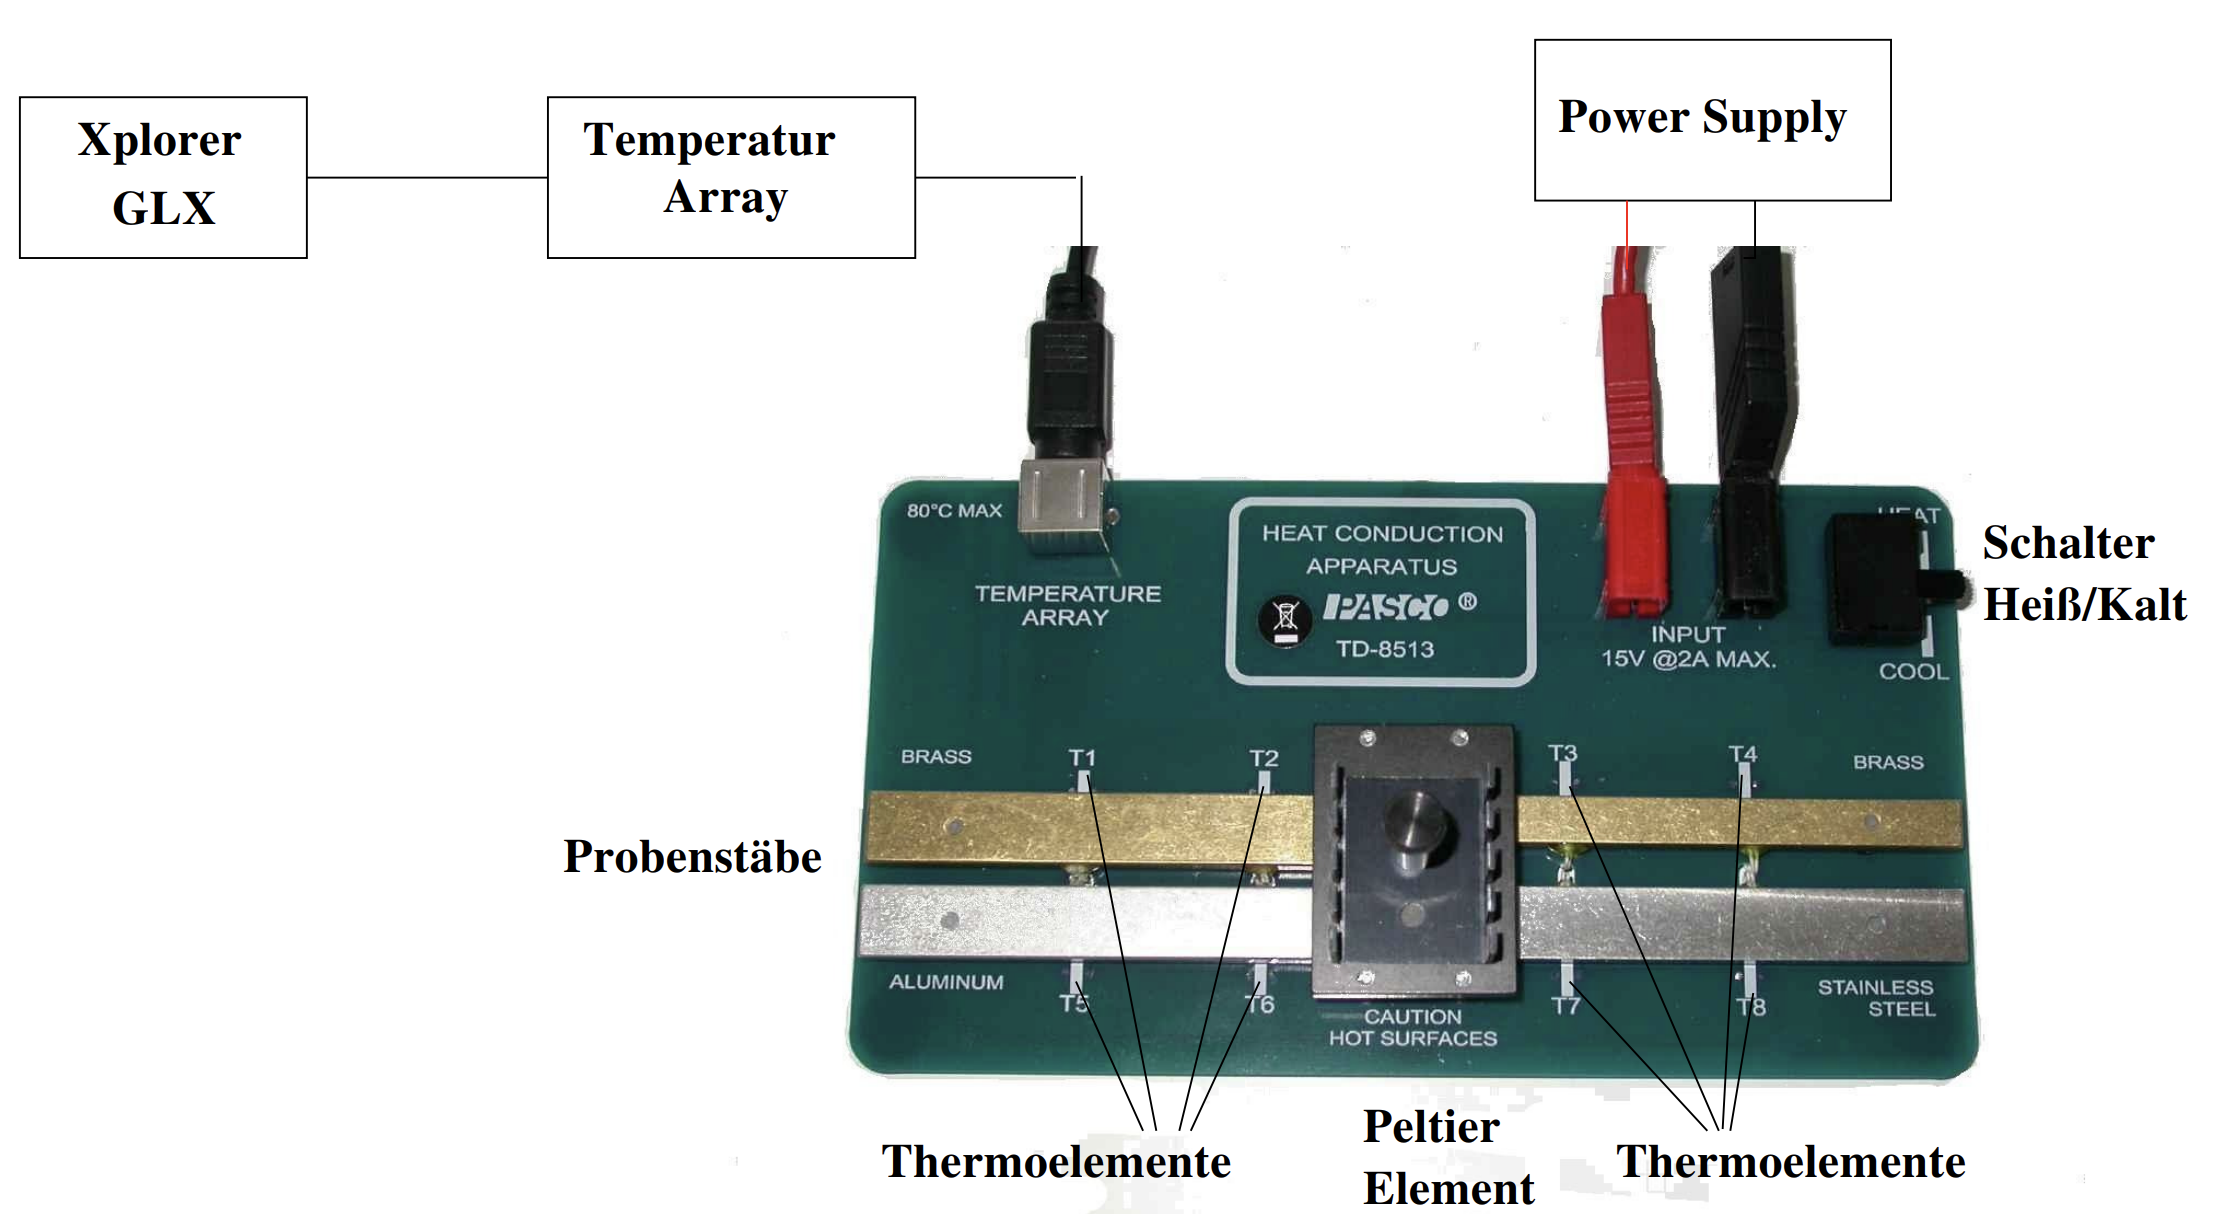
\includegraphics[width=\textwidth]{placeholder.png}
    \caption{Ent- und Aufladung eines Kondensators über einen Widerstand}
\end{figure}

\subsection{Relaxationsvorgänge durch periodische Auslenkung}

\subsection{Die Funktion des RC-Kreises als Integrator}


\section{Fehlerrechnung}
\end{document}